\section{Secure Remote Access to Routers through SSH}
\label{sec:ssh}

\subsection{Design}

Accessing the routers through the physical "console" port is inconvenient and dangerous. Thus, remote acess through Secure Shell (SSH) protocol\citep{rfc4253} to routers is needed. 

In BT network, remote SSH access is enabled on all 3 routers. Seperate combinations of username and password on each router are used to ensure the independence of security of each router.

In addition, SSH public key authentication is set up on Laptop 1 (BT001), which allows the root user on the laptop to login in to all routers without entering passwords.

\subsection{Implementation}

We first set up Remote SSH access was first set up as instructed in Reference Guide on all 3 routers. Below is the configuration commands for Router 1 (BT-R001).

\begin{lstlisting}
hostname BT-R001
ip domain name bt.lboro
username r001 priv 15 secret <secret>
line vty 0 4
transport input ssh telnet
login local

ip ssh version 2
crypto key generate rsa general-keys
ip ssh dh min size 4096
\end{lstlisting}

We then generate a pair of public and private keys on Laptop 1 (BT001).

\begin{lstlisting}
ssh-keygen
\end{lstlisting}

After that, the pair of keys is written into files
\texttt{\textasciitilde{}/.ssh/id\_rsa} and
\texttt{\textasciitilde{}/.ssh/id\_rsa.pub} . We use the generated
public key ( \texttt{id\_rsa.pub} ) to set up SSH public key
authentication on all 3 routers.

\begin{lstlisting}
ip ssh pubkey-chain
username r001
key-string
\end{lstlisting}

\subsection{Evaluation}

Once remote SSH access is set up on 3 routers, one should be able to access them on Laptop 1 (BT001) without entering the password using the following commands.

\begin{lstlisting}[language=sh]
# access Router 1
ssh r001@23.0.0.1 
# access Router 2
ssh r002@23.0.0.50
# access Router 3
ssh r003@23.0.0.33
\end{lstlisting}

Screenshots of successful remote access to all $3$ routers are shown in Figure \ref{fig:ssh}.

\begin{figure*}[ht!]
    \centering
    \begin{subfigure}[b]{0.67\textwidth}
        \centering
        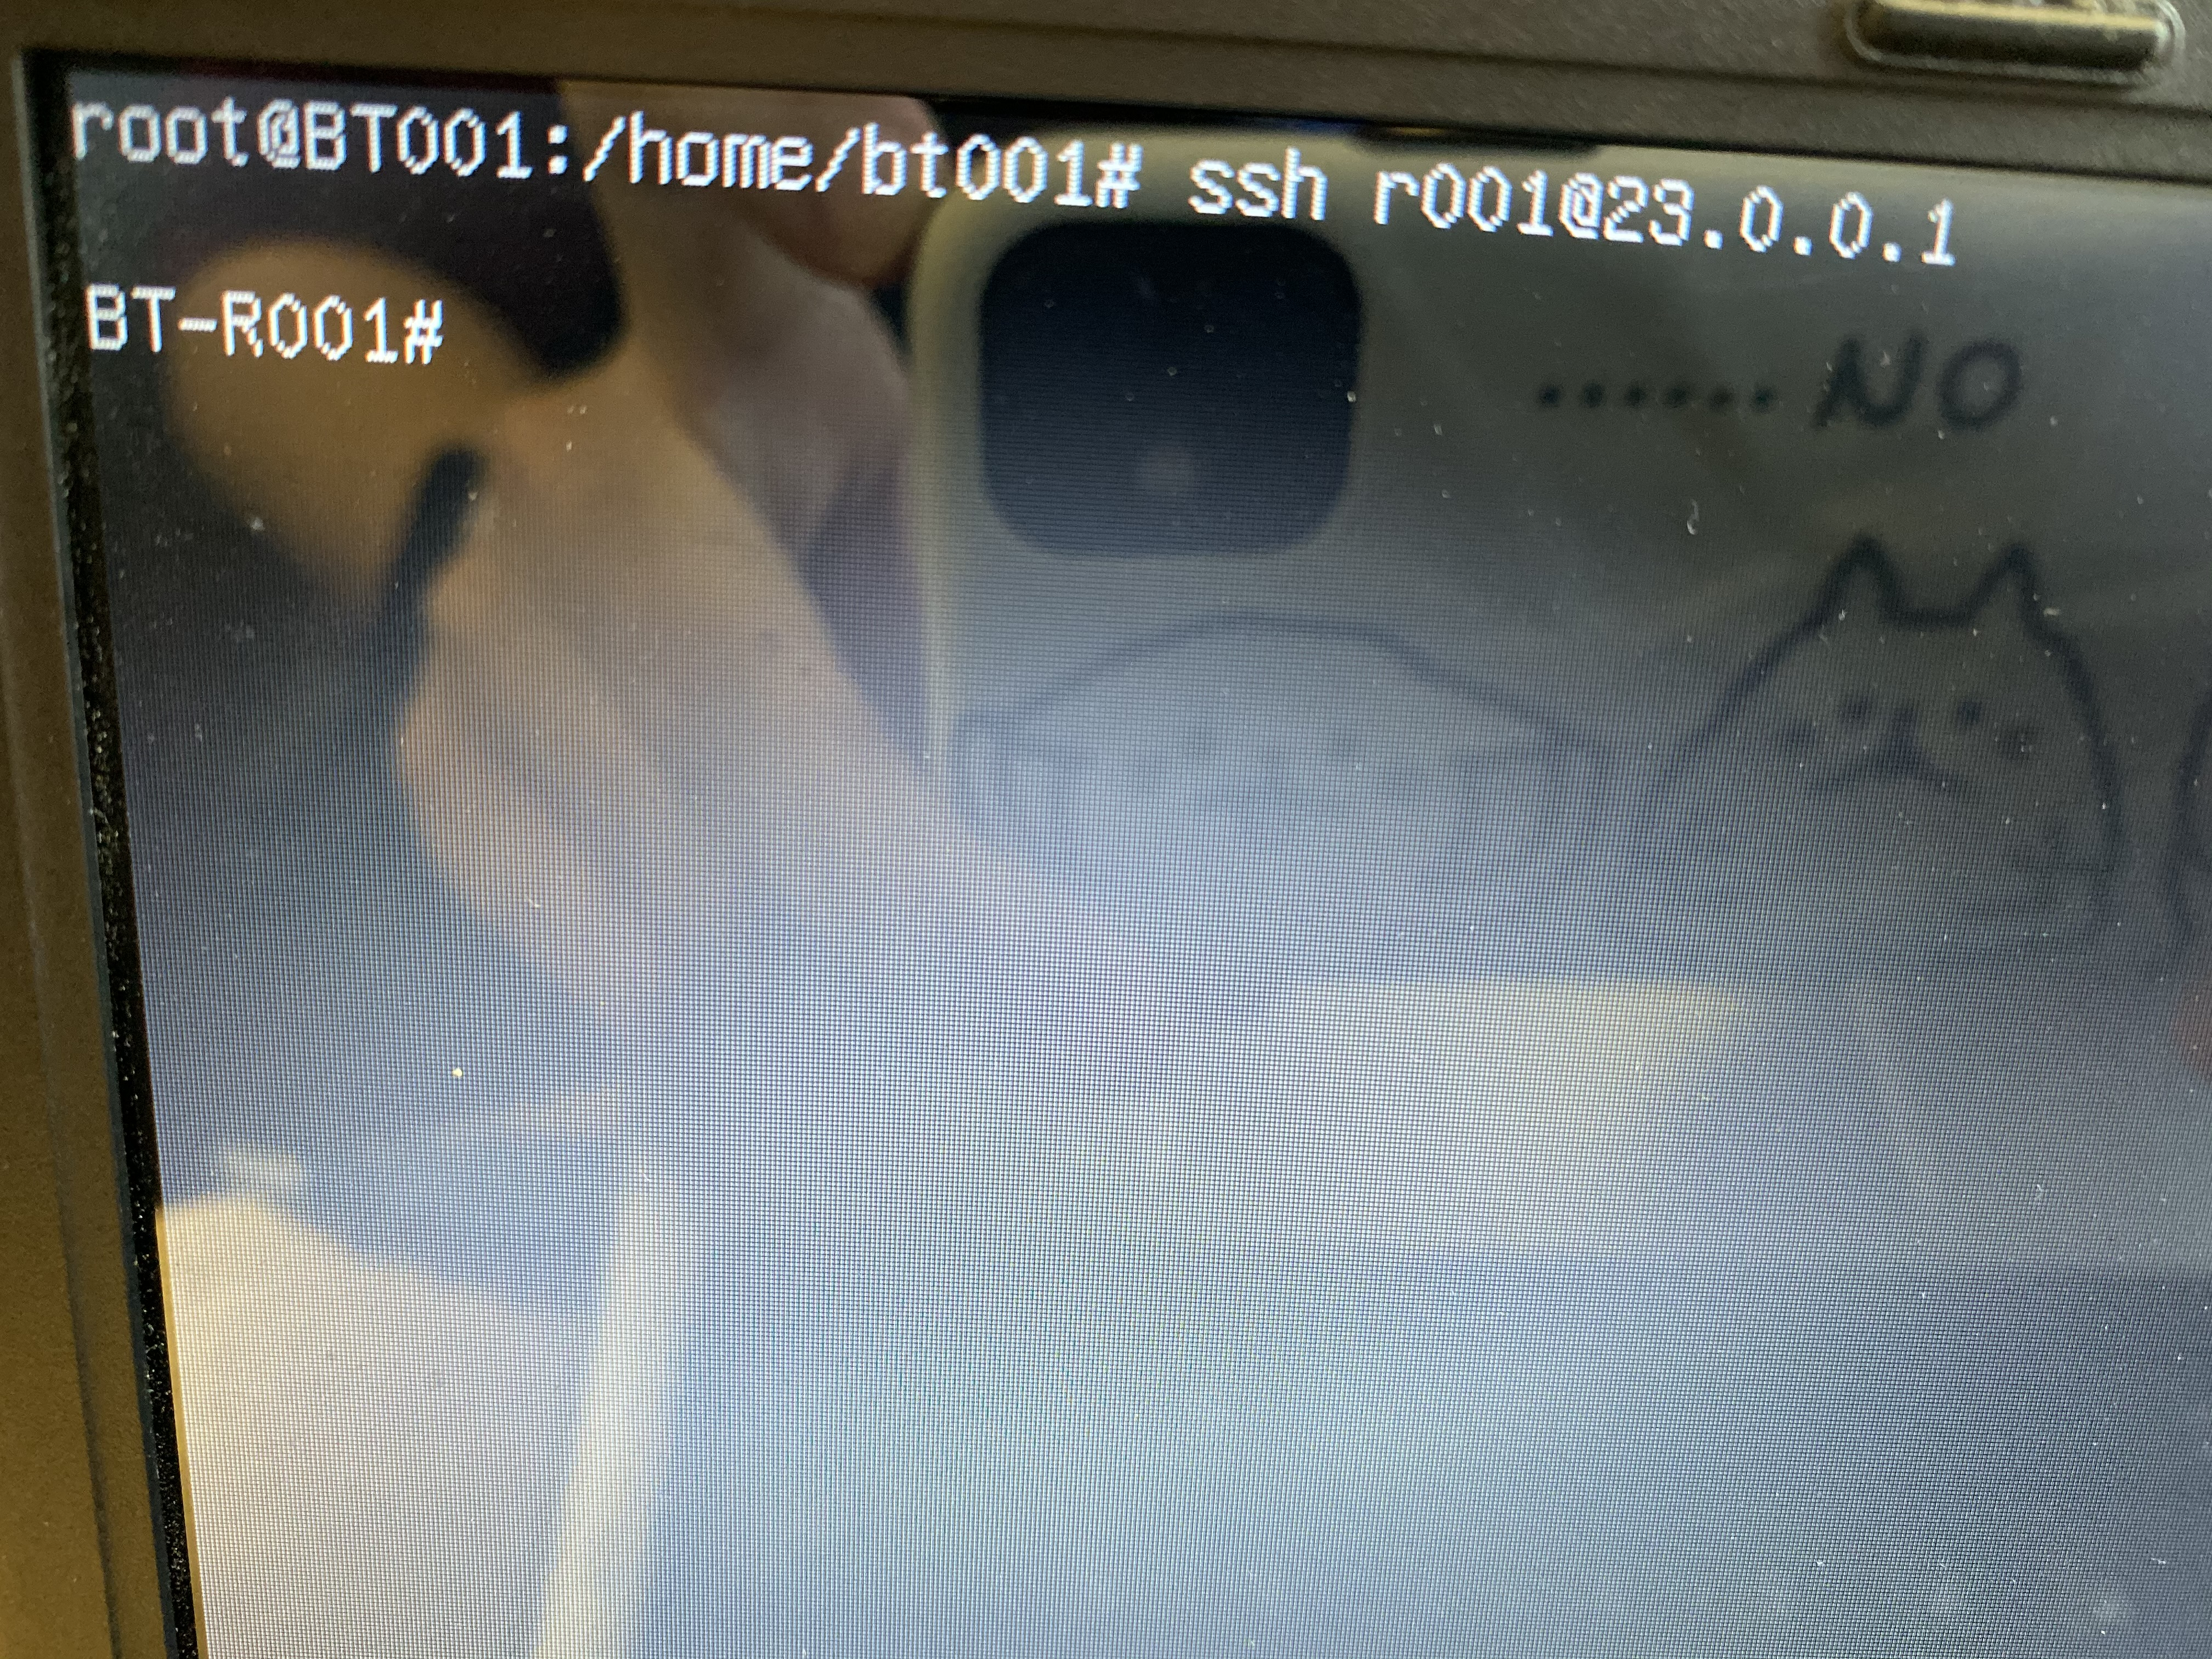
\includegraphics[width=\linewidth]{ssh1}
        \caption{Router 1 (BT-R001)}
    \end{subfigure}
    \hfill
    \begin{minipage}[b]{0.3\textwidth}
	    \begin{subfigure}[b]{\linewidth}
	        \centering
	        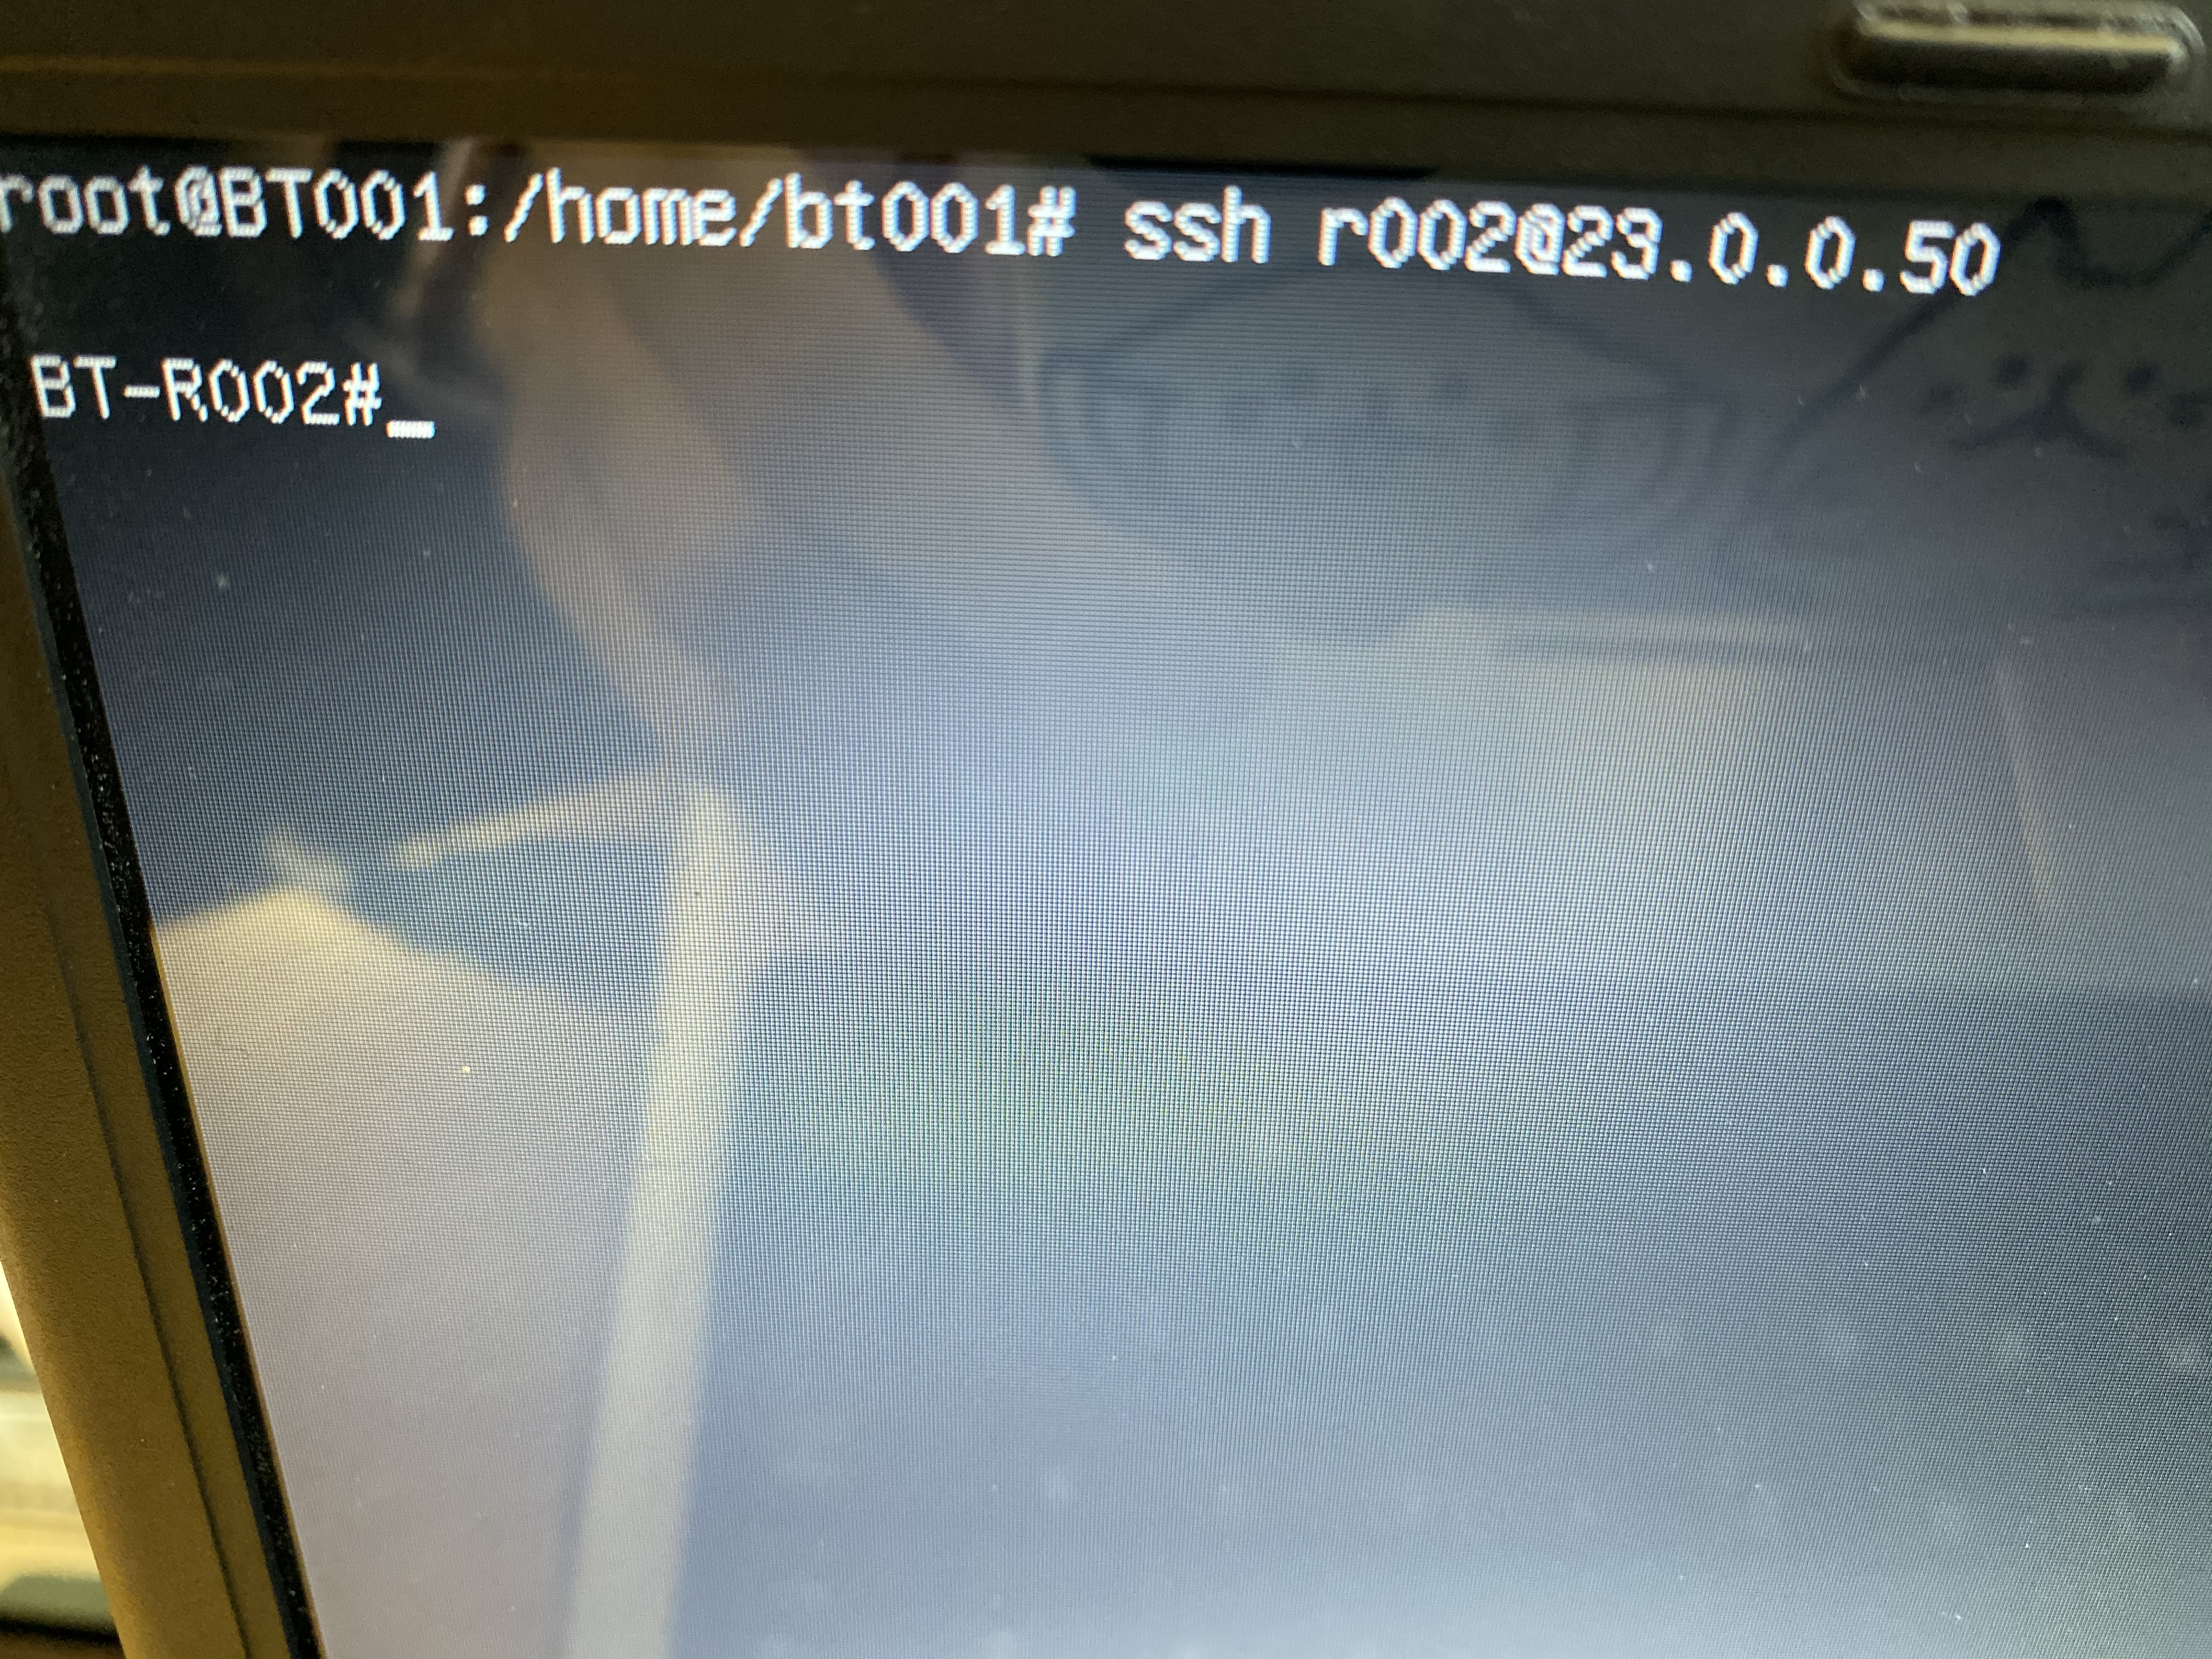
\includegraphics[width=\linewidth]{ssh2}
	        \caption{Router 2 (BT-R002)}
	    \end{subfigure}
	    \\
	    \begin{subfigure}[b]{\linewidth}
	        \centering
	        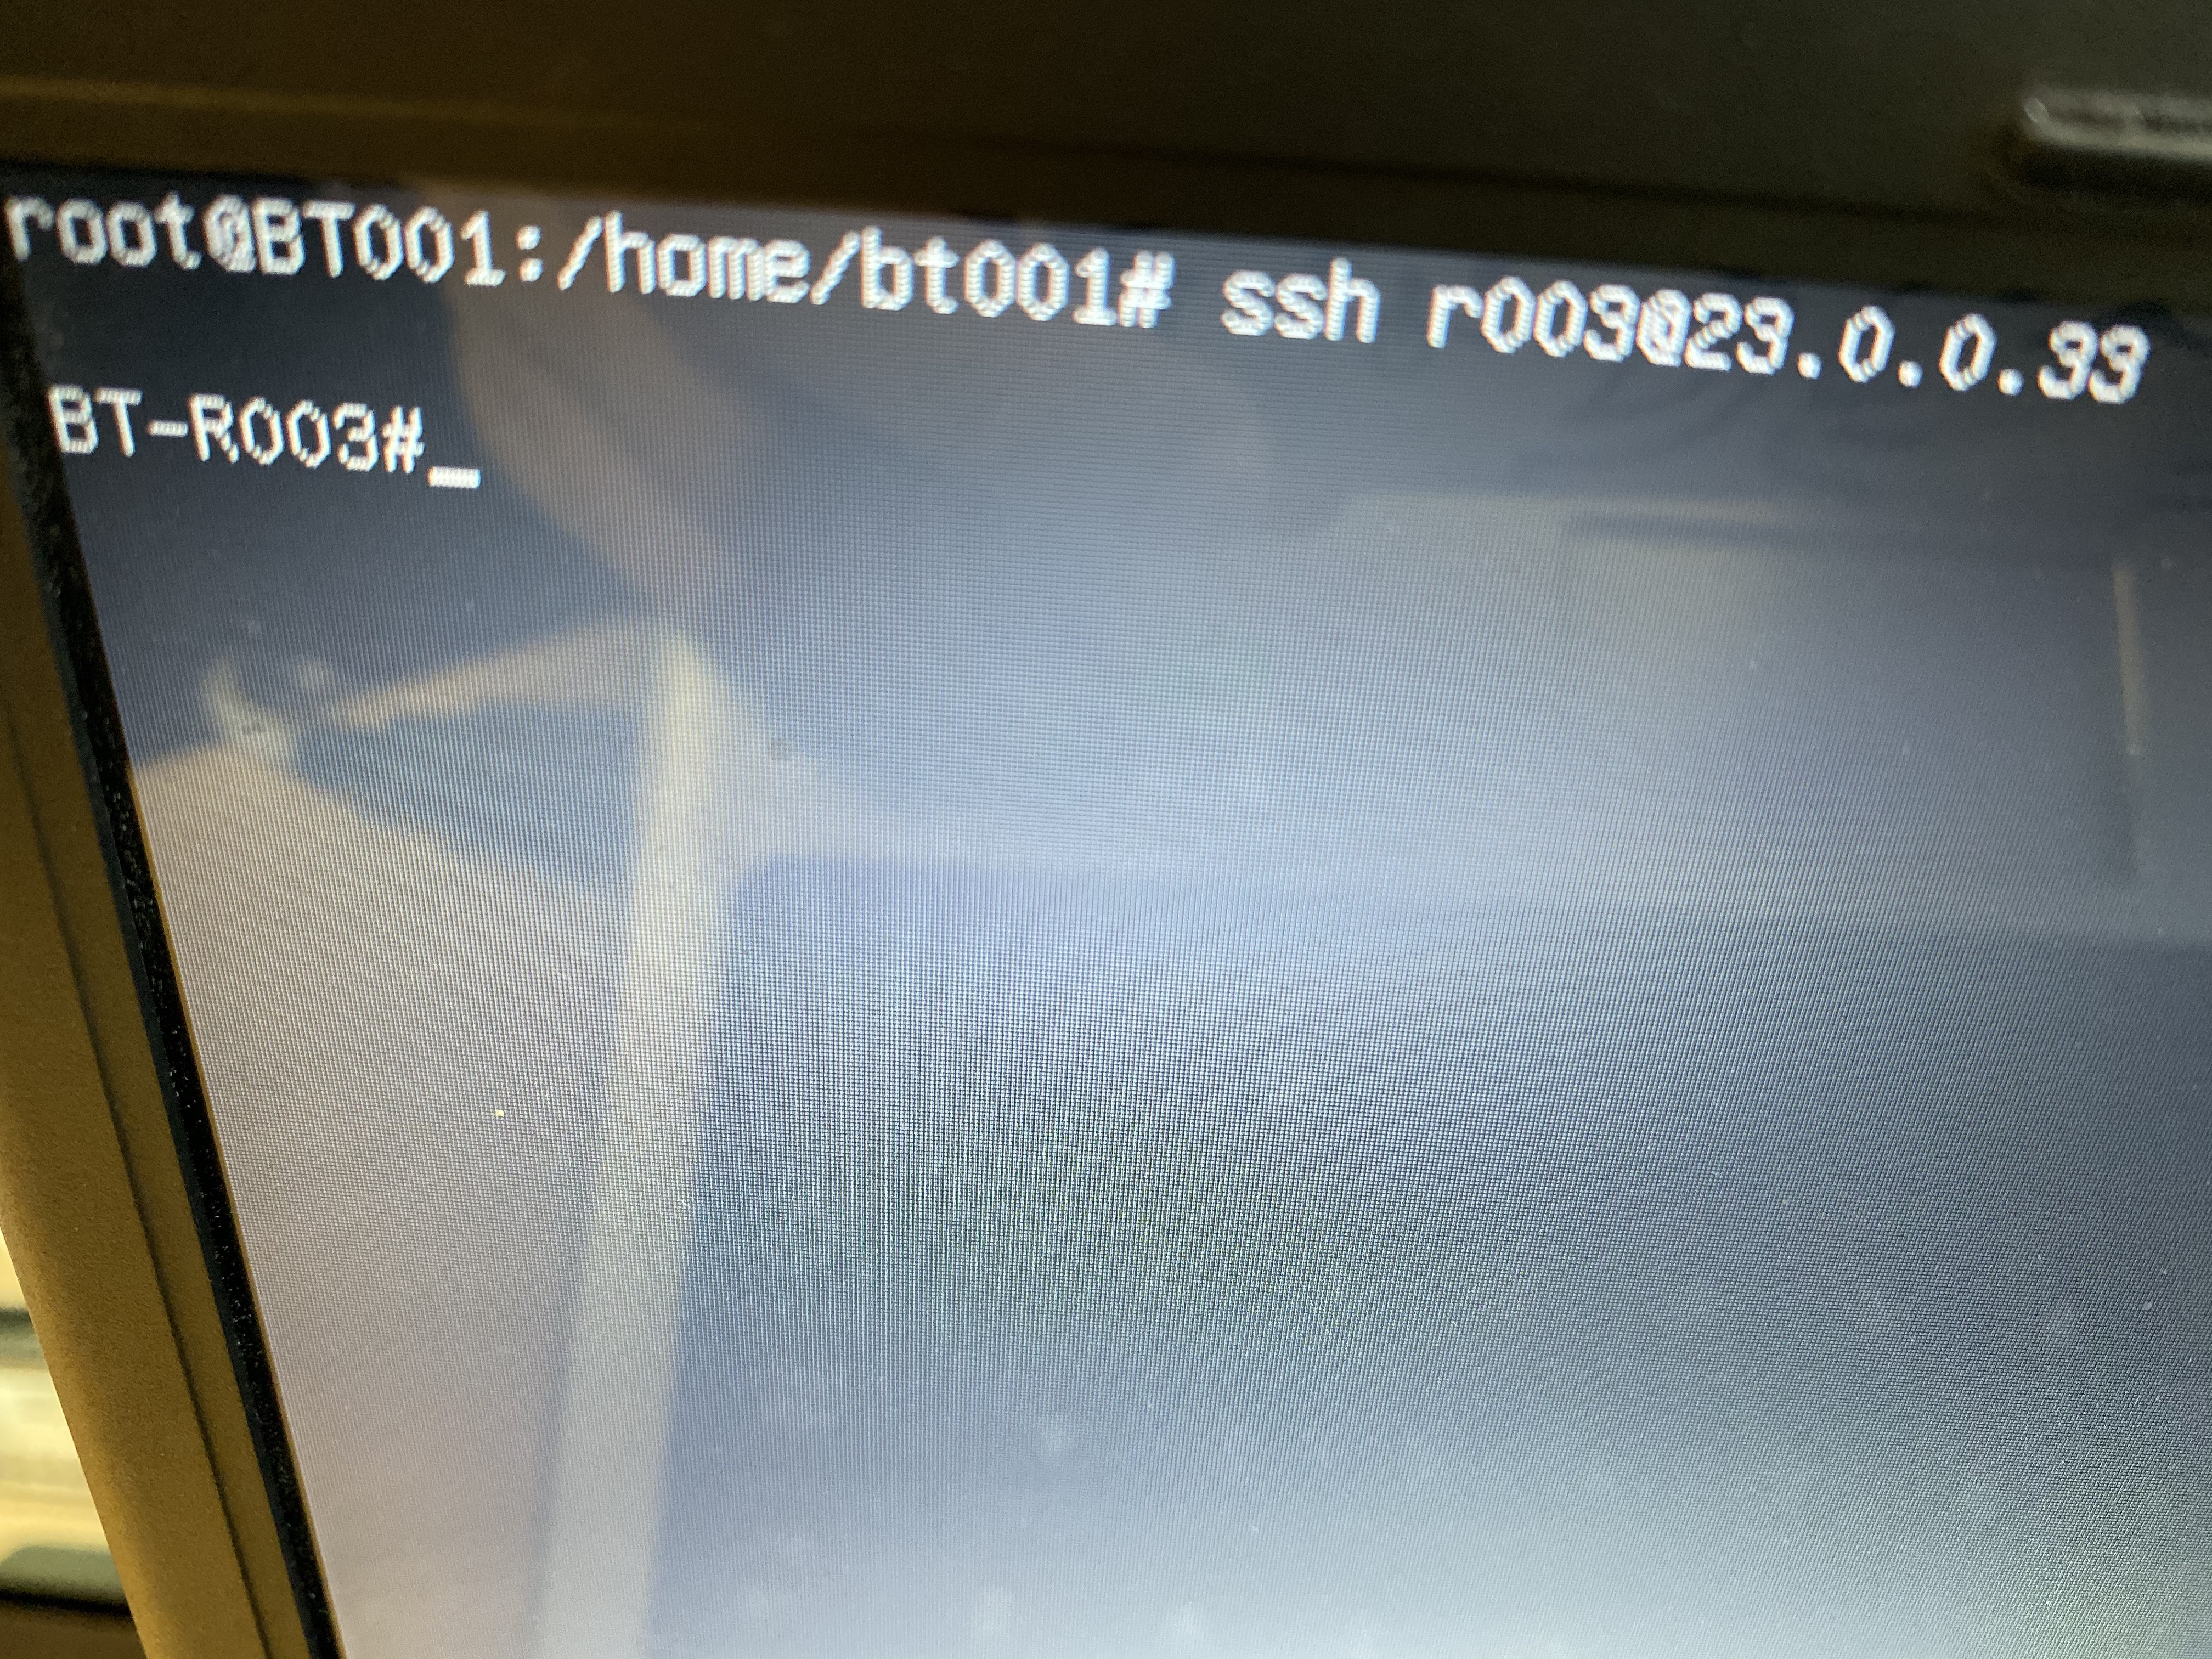
\includegraphics[width=\linewidth]{ssh3}
	        \caption{Router 3 (BT-R003)}
	    \end{subfigure}
	\end{minipage}
    \caption{Sucessful remote SSH access to all 3 routers from Laptop 1 (BT001).}
    \label{fig:ssh}
\end{figure*}

% \begin{figure*}[t!]
%     \centering
%     \begin{subfigure}[t]{0.3\textwidth}
%         \centering
%         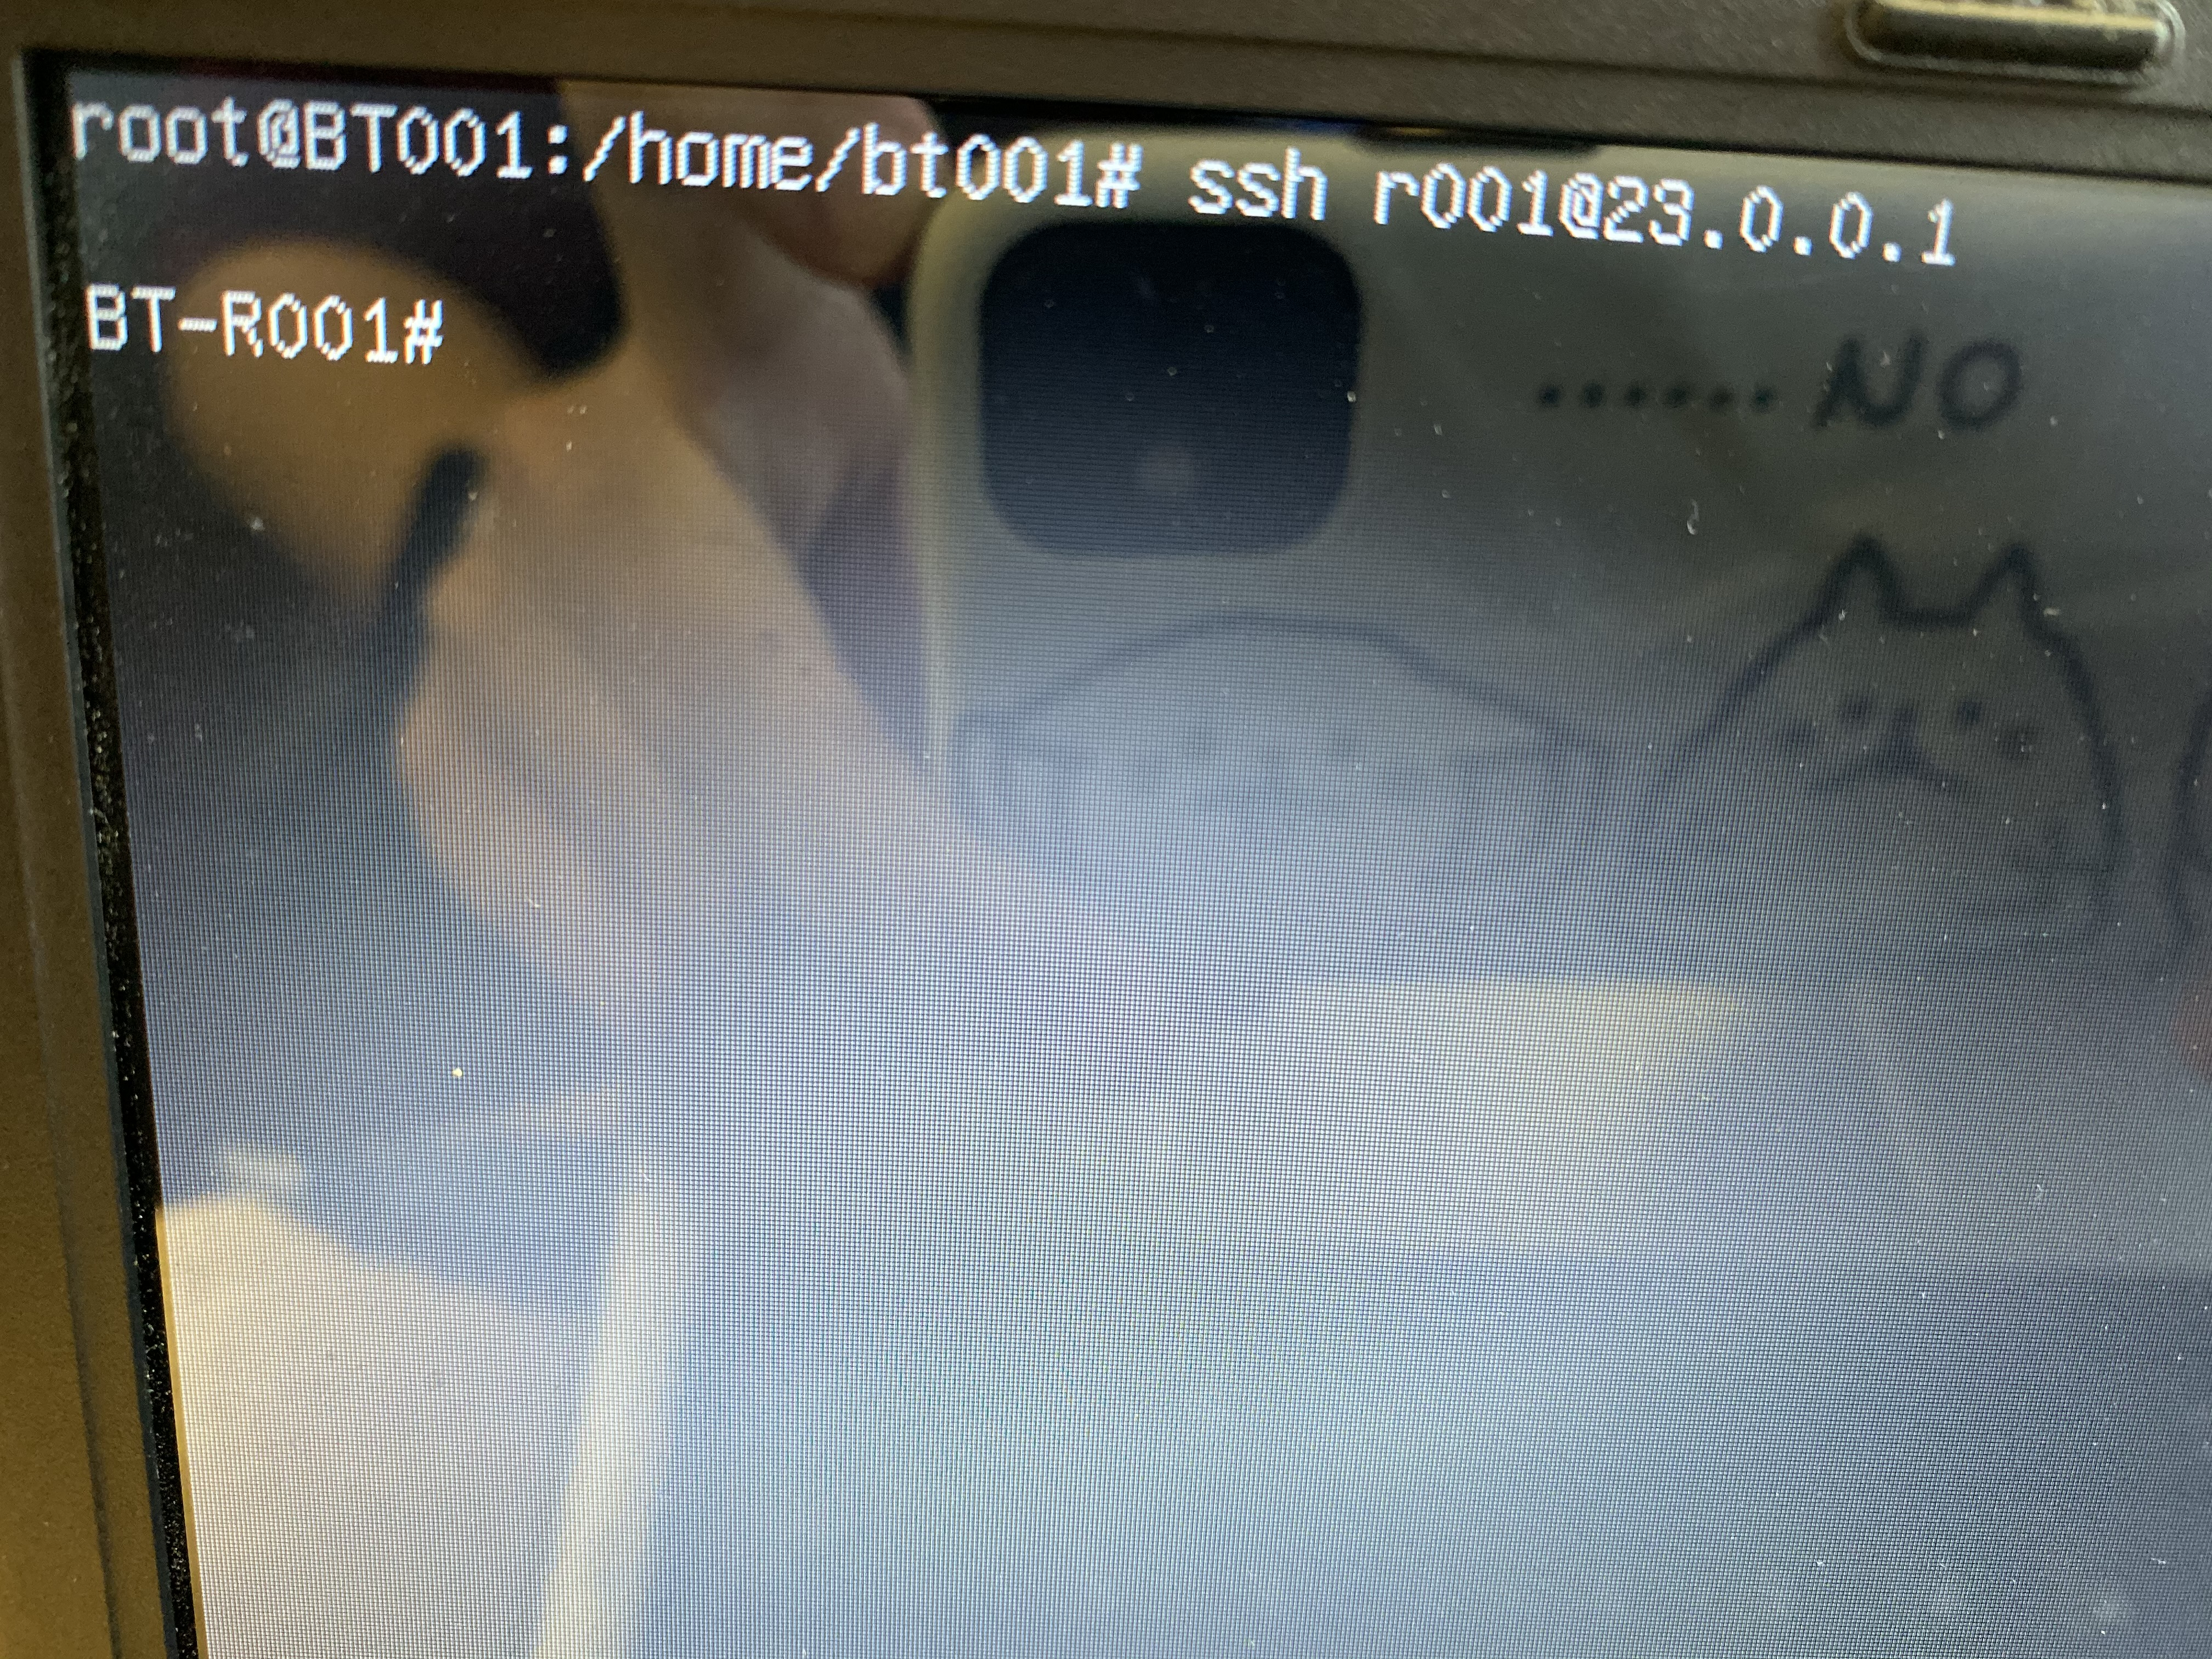
\includegraphics[width=\linewidth]{ssh1}
%         \caption{Router 1 (BT-R001)}
%     \end{subfigure}
%     ~ 
%     \begin{subfigure}[t]{0.3\textwidth}
%         \centering
%         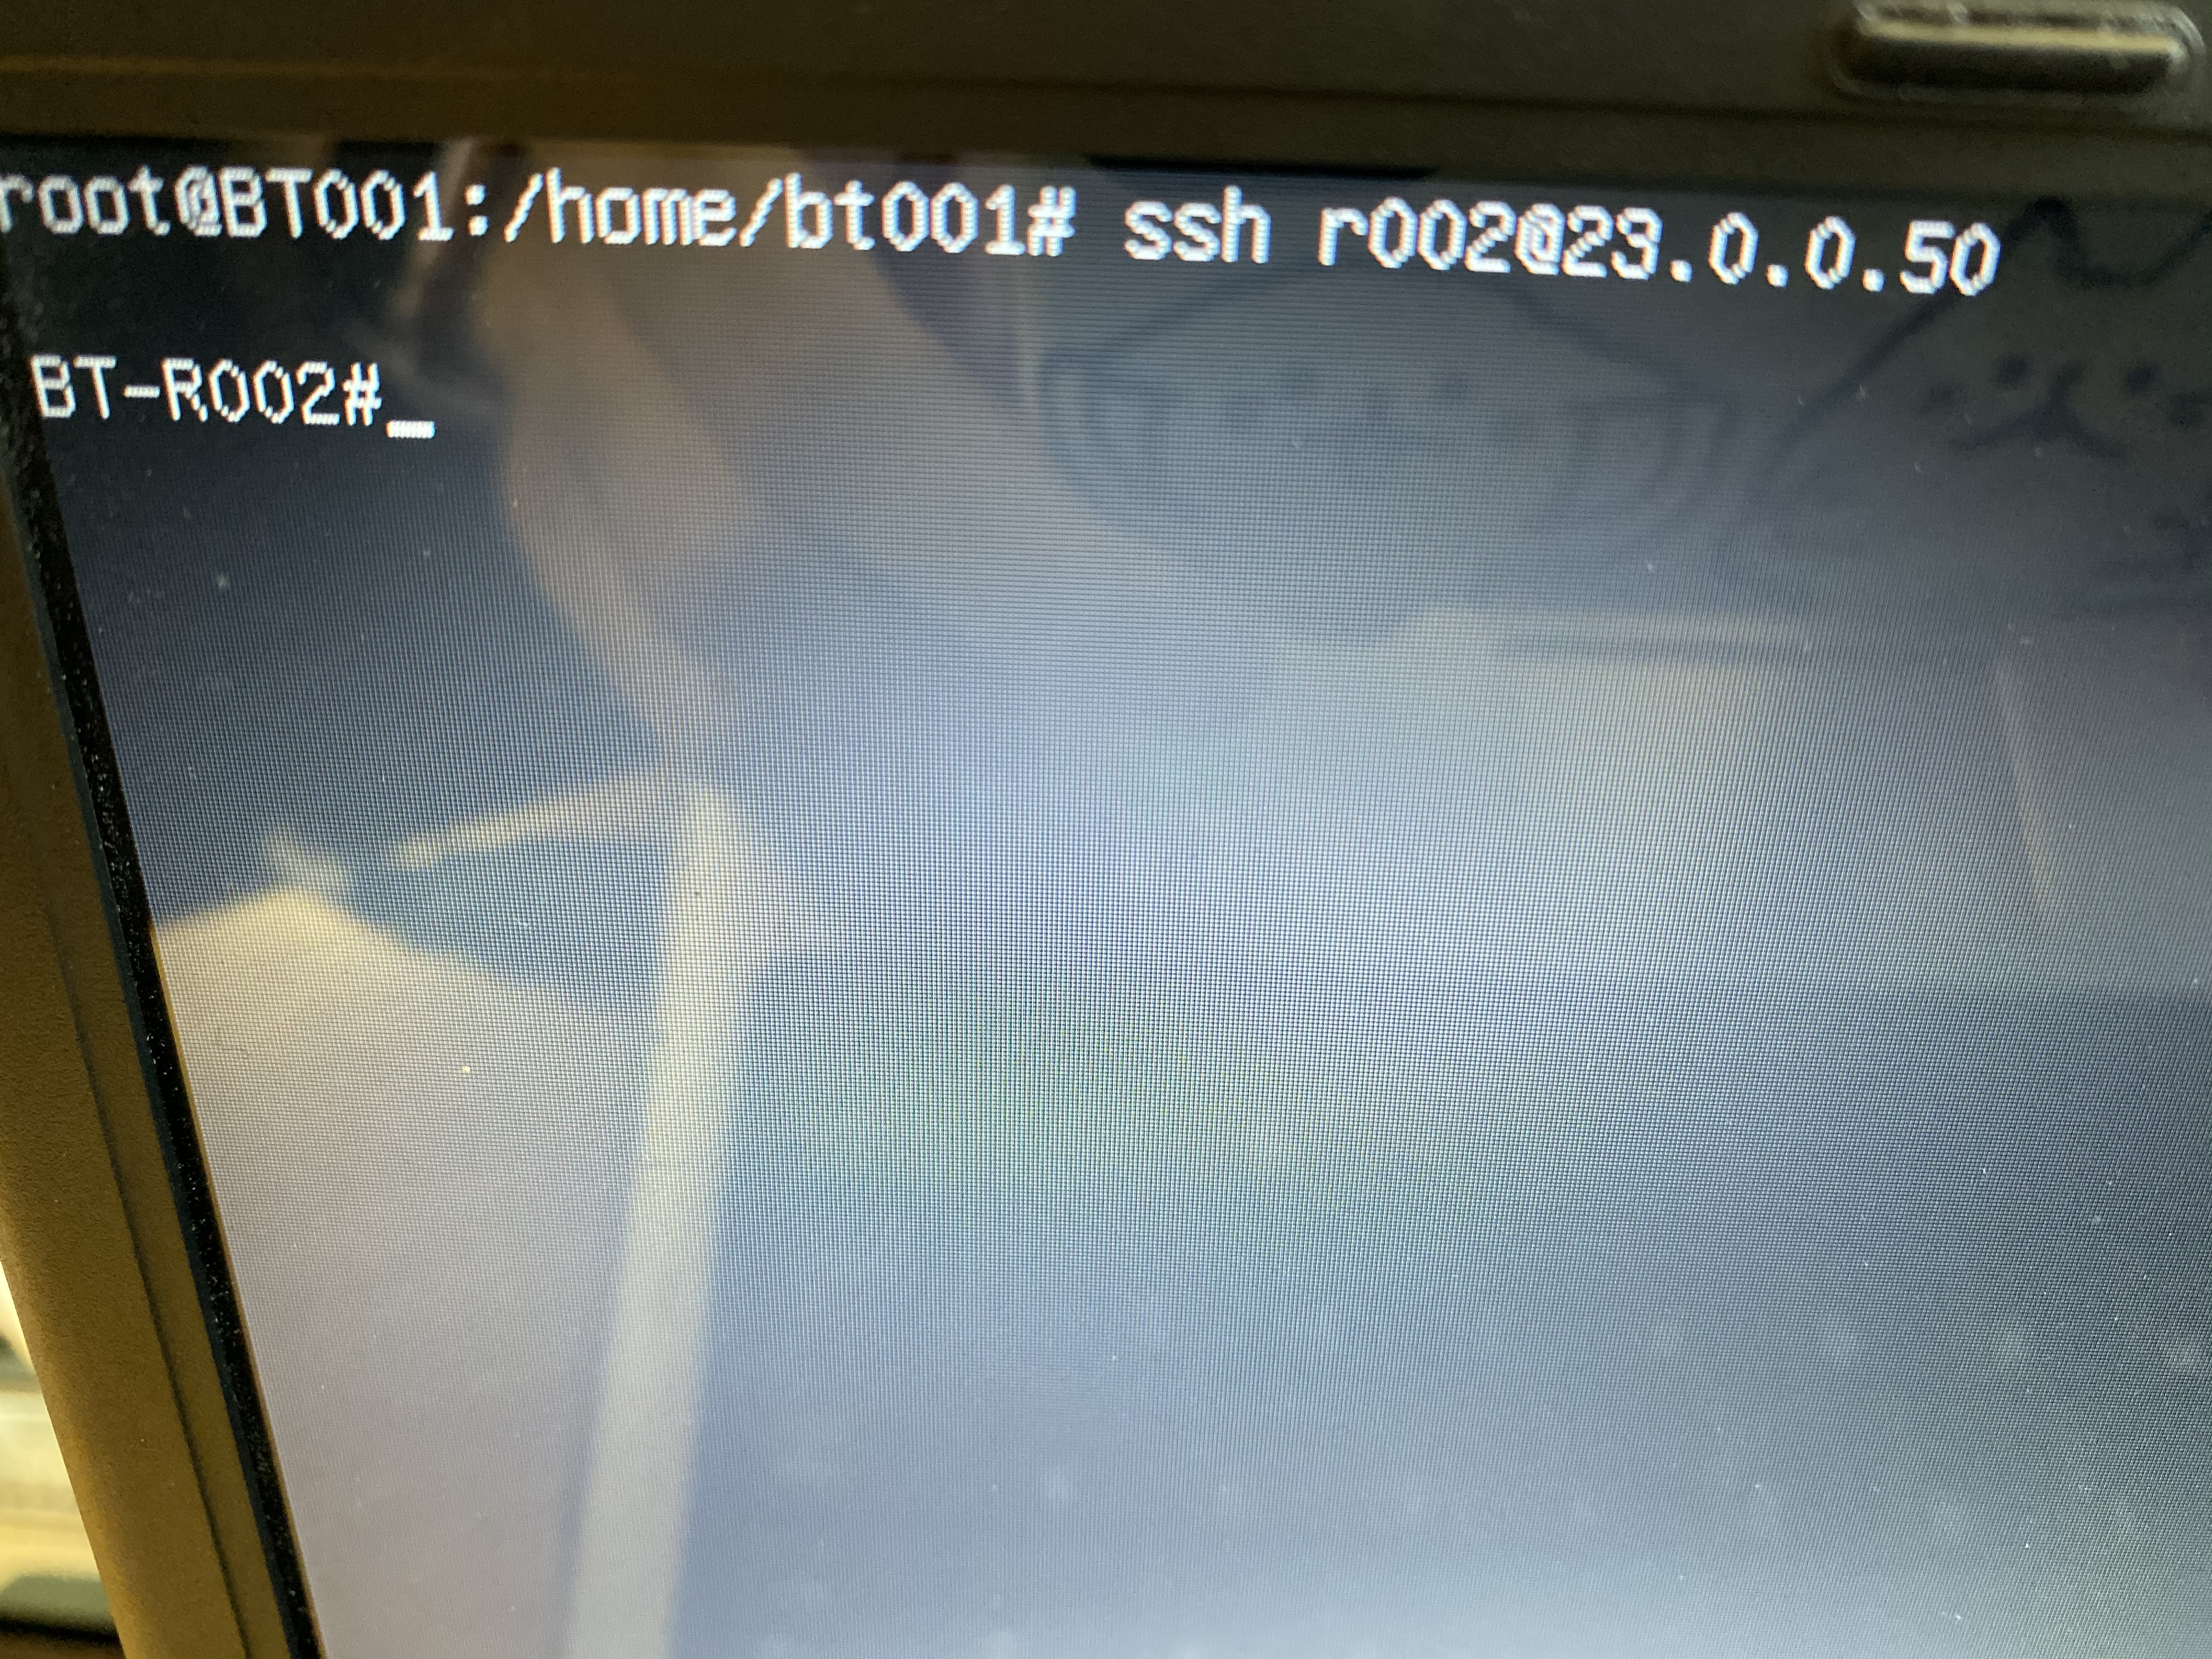
\includegraphics[width=\linewidth]{ssh2}
%         \caption{Router 2 (BT-R002)}
%     \end{subfigure}
%     ~ 
%     \begin{subfigure}[t]{0.3\textwidth}
%         \centering
%         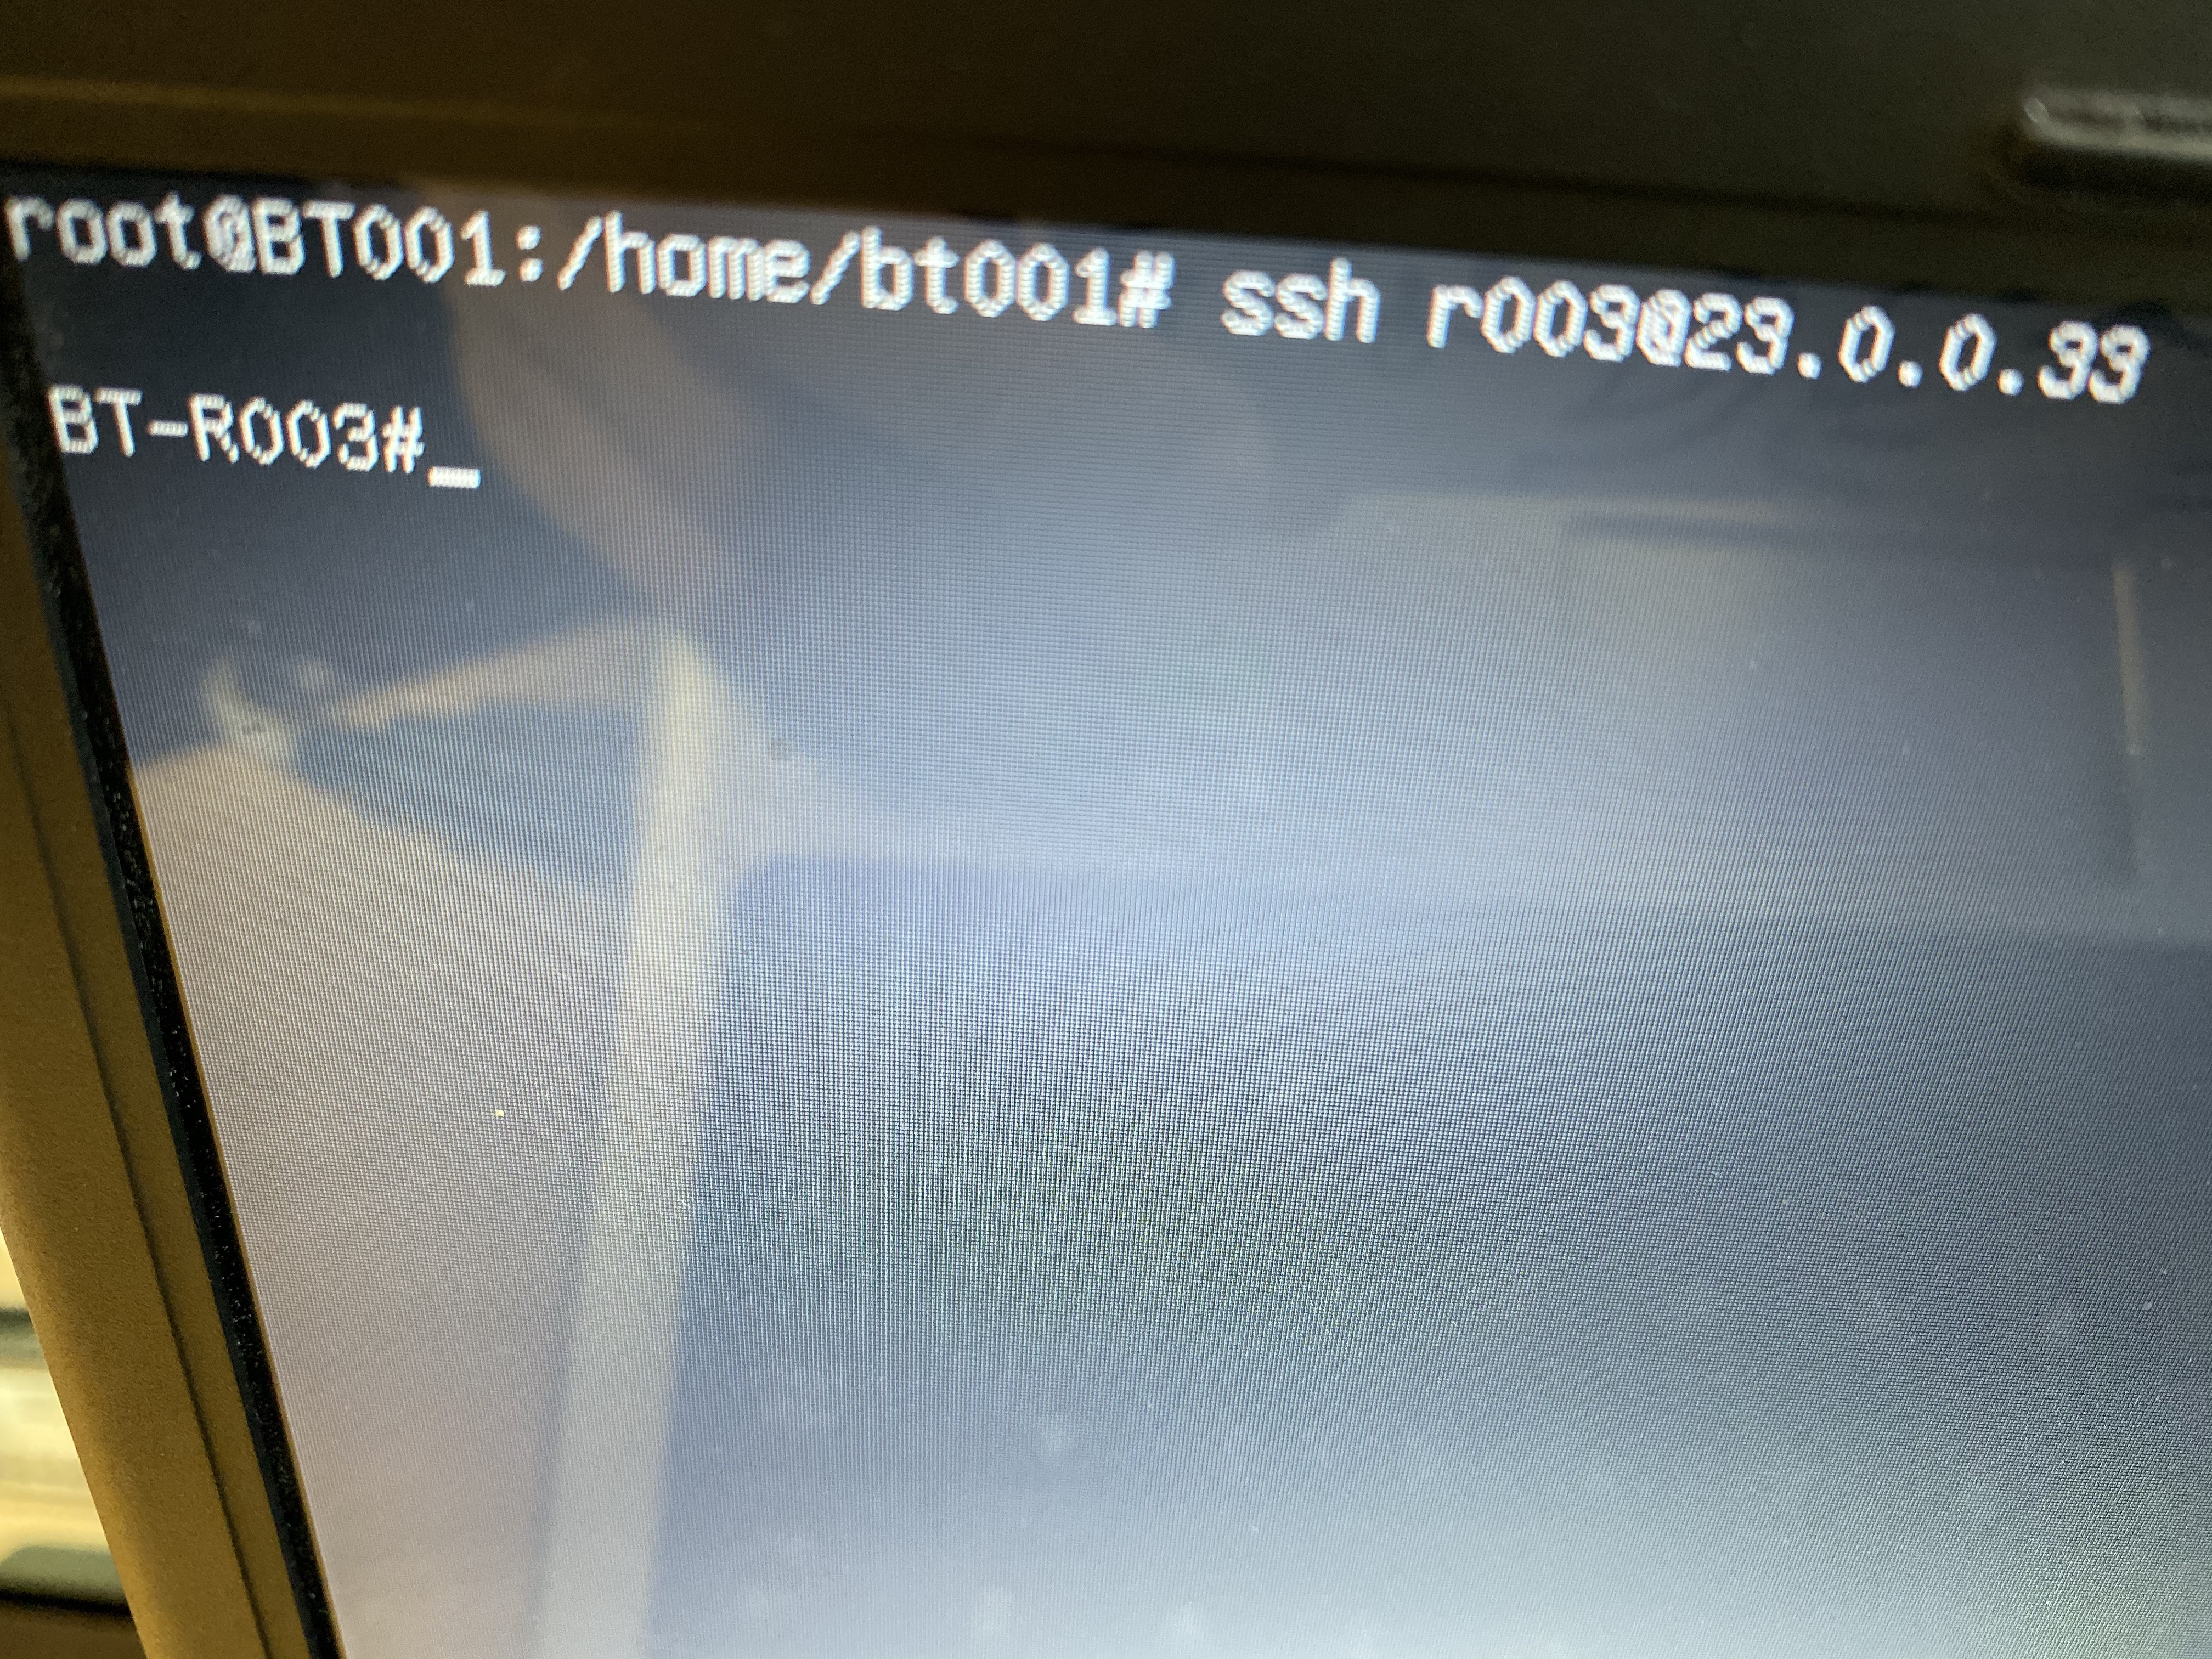
\includegraphics[width=\linewidth]{ssh3}
%         \caption{Router 3 (BT-R003)}
%     \end{subfigure}
%     \caption{Sucessful remote SSH access to all 3 routers from Laptop 1 (BT001).}
%     \label{fig:ssh}
% \end{figure*}


\subsection{Commentary}

\subsubsection{Problem: Maximum Limit of Characters per Line}

When we tried to set up SSH public key authentication on routers, we failed at our initial attempt. It turned out that Cisco router has maximum limit of characters for each command line. Thus, a public key in a single long line was not accepted by the router. 

To solve this problem, \texttt{fold} command is used to split the public key into multiple lines before re-uploading the key and SSH public key authentication was successfully set up on the router.
